%%%%%%%%%%%%%%%%%%%%%%%%%%%%%%%%%%%%%%%%%%%%%%%%%%%%%%%%%%%%%%%
%
% Welcome to Overleaf --- just edit your article on the left,
% and we'll compile it for you on the right. If you give 
% someone the link to this page, they can edit at the same
% time. See the help menu above for more info. Enjoy!
%
%%%%%%%%%%%%%%%%%%%%%%%%%%%%%%%%%%%%%%%%%%%%%%%%%%%%%%%%%%%%%%%
%
% For more detailed article preparation guidelines, please see: http://wellcomeopenresearch.org/for-authors/article-guidelines and http://wellcomeopenresearch.org/for-authors/data-guidelines

\documentclass[10pt,a4paper,twocolumn]{article}
\usepackage{WellcomeOR_styles}

%% Default: numerical citations
\usepackage[numbers]{natbib}

%% Uncomment this lines for superscript citations instead
% \usepackage[super]{natbib}

%% Uncomment these lines for author-year citations instead
% \usepackage[round]{natbib}
% \let\cite\citep

\usepackage{hyperref}

\begin{document}

\def\partitle{Pre-vaccination testing could expand coverage of 2-dose COVID vaccines}

\author[1,2,*]{Carl A. B. Pearson}
\author[1]{Sam Clifford}
\author[2]{Juliet R. C. Pulliam}
\author[1]{\mbox{Rosalind} M. Eggo}
\affil[1]{Department of Infectious Disease Epidemiology \&\ Centre for Mathematical Modelling of Infectious Diseases,
London School of Hygiene \&\ Tropical Medicine

Keppel Street, London, United Kingdom WC1E 7HT

\{carl.pearson, sam.clifford, r.eggo\}@lshtm.ac.uk}
\affil[2]{DSI-NRF Centre of Excellence in Epidemiological Modelling and Analysis, Stellenbosch University

19 Jonkershoek Road, Stellenbosch, South Africa, 7600

pulliam@sun.ac.za
}
\affil[*]{corresponding}
\title{\partitle}
%\titlenote{The title should be detailed enough for someone to know whether the article would be of interest to them, but also concise. Please ensure the broadness and claims within the title are appropriate to the content of the article itself.}

\maketitle
\thispagestyle{fancy}

%Please list all authors that played a significant role in the research involved in the article. Please provide full affiliation information (including full institutional address, ZIP code and e-mail address) for all authors, and identify who is/are the corresponding author(s).

\newcommand{\eref}[1]{Eq.~\ref{#1}}
\newcommand{\fref}[1]{Fig.~\ref{#1}}
\newcommand{\sref}[1]{Section~\ref{#1}}
\newcommand{\srefs}[1]{Sections~\ref{#1}}

\newcommand{\dPois}[1]{\sim \textrm{Pois}(#1)}

% \def\name{definition} here
\def\eg*{\textit{e.g.}}
\def\ie*{\textit{i.e.}}
\def\nb*{\textit{n.b.}}
\def\etc*{\textit{etc.}}

\def\TPR{\textrm{TPR}}
\def\TNR{\textrm{TNR}}
\def\FPR{\textrm{FPR}}
\def\FNR{\textrm{FNR}}

\def\PPD{\textrm{PPD}}
\def\CPP{\textrm{CPP}}
\def\CPD{\textrm{CPD}}

\def\rhop{\rho_{{+}}}
\def\rhon{\rho_{{-}}}

\newcommand{\abs}[1]{\lvert #1\rvert}

\begin{abstract}

Recent evidence indicates that a single dose of mRNA-based vaccines produce similar immune responses in people with evidence of past infection compared with two doses in immunologically naive individuals. For COVID-19 vaccines with two dose regimens, point-of-care antibody testing for prior infection when administering the first dose could enable expanded vaccine access in a cost-effective manner. Generally, antibody tests with sensitivity and specificity well below that typically accepted for product licensure would still enable expanded vaccine coverage, though to be cost-beneficial total (\ie* procurement and administration) test cost needs to be less than roughly a third of total vaccine dose cost. For highly sensitive (90\%) and specific (99\%) tests, coverage could be expanded by more than 33\%. Tests with the appropriate performance characteristics are plausible, though likely need setting specific tailoring.

\end{abstract}

\section*{Keywords}

COVID-19, SARS-CoV-2, Vaccination, Point-of-Care Antibody Testing, Rapid Serological Testing

\clearpage


\section*{Introduction}

Many countries have experienced high SARS-CoV-2 infection attack rates and currently have limited vaccine supplies. For example, countries participating in the COVAX facility expect to receive vaccine coverage for only 20\% of their populations \cite{noauthor_gavi_nodate}, with any additional coverage depending on availability and cost. However, recent evidence indicates that a single dose of the mRNA-based vaccines (\eg* the Pfizer or Moderna products) produce immune responses in people with evidence of past infection (\ie* seropositive) that are at least comparable to the response elicited by two doses in immunologically naive individuals \cite{krammer_antibody_2021,stamatatos_mrna_2021,samanovic_poor_2021,saadat_binding_2021,lustig_neutralizing_2021}.

If effects observed in these studies are validated, the use of a point-of-care antibody test when administering the first dose could allow for more efficient use of available vaccine doses. This benefit depends on test performance, cost, and the seroprevalence in the population being vaccinated. Intuitively, the advantage will increase with greater seroprevalence because there is more opportunity to reallocate the second dose. To be a better option than buying more doses, administering a test should cost less than a single vaccine dose, but how much less will depend on test specificity (to avoid giving too few doses) and sensitivity (to benefit from reallocating doses), as well as seroprevalence. Several rapid, point-of-care antibody tests \cite{baraniuk_covid-19_2020,mathur_antibody_2020,shuren_fdas_2021,prazuck_evaluation_2021} are available that may ultimately be able meet these requirements, however further testing and development may be needed to validate and tailor tests for use in different contexts \cite{ndaye_challenges_2021,tso_high_2021,emmerich_limited_2021}. Data to evaluate vaccine effectiveness for a single dose conditional on antibody testing could be collected in countries pursuing a delayed second dose scheme, like the United Kingdom.

\begin{figure}
\centering
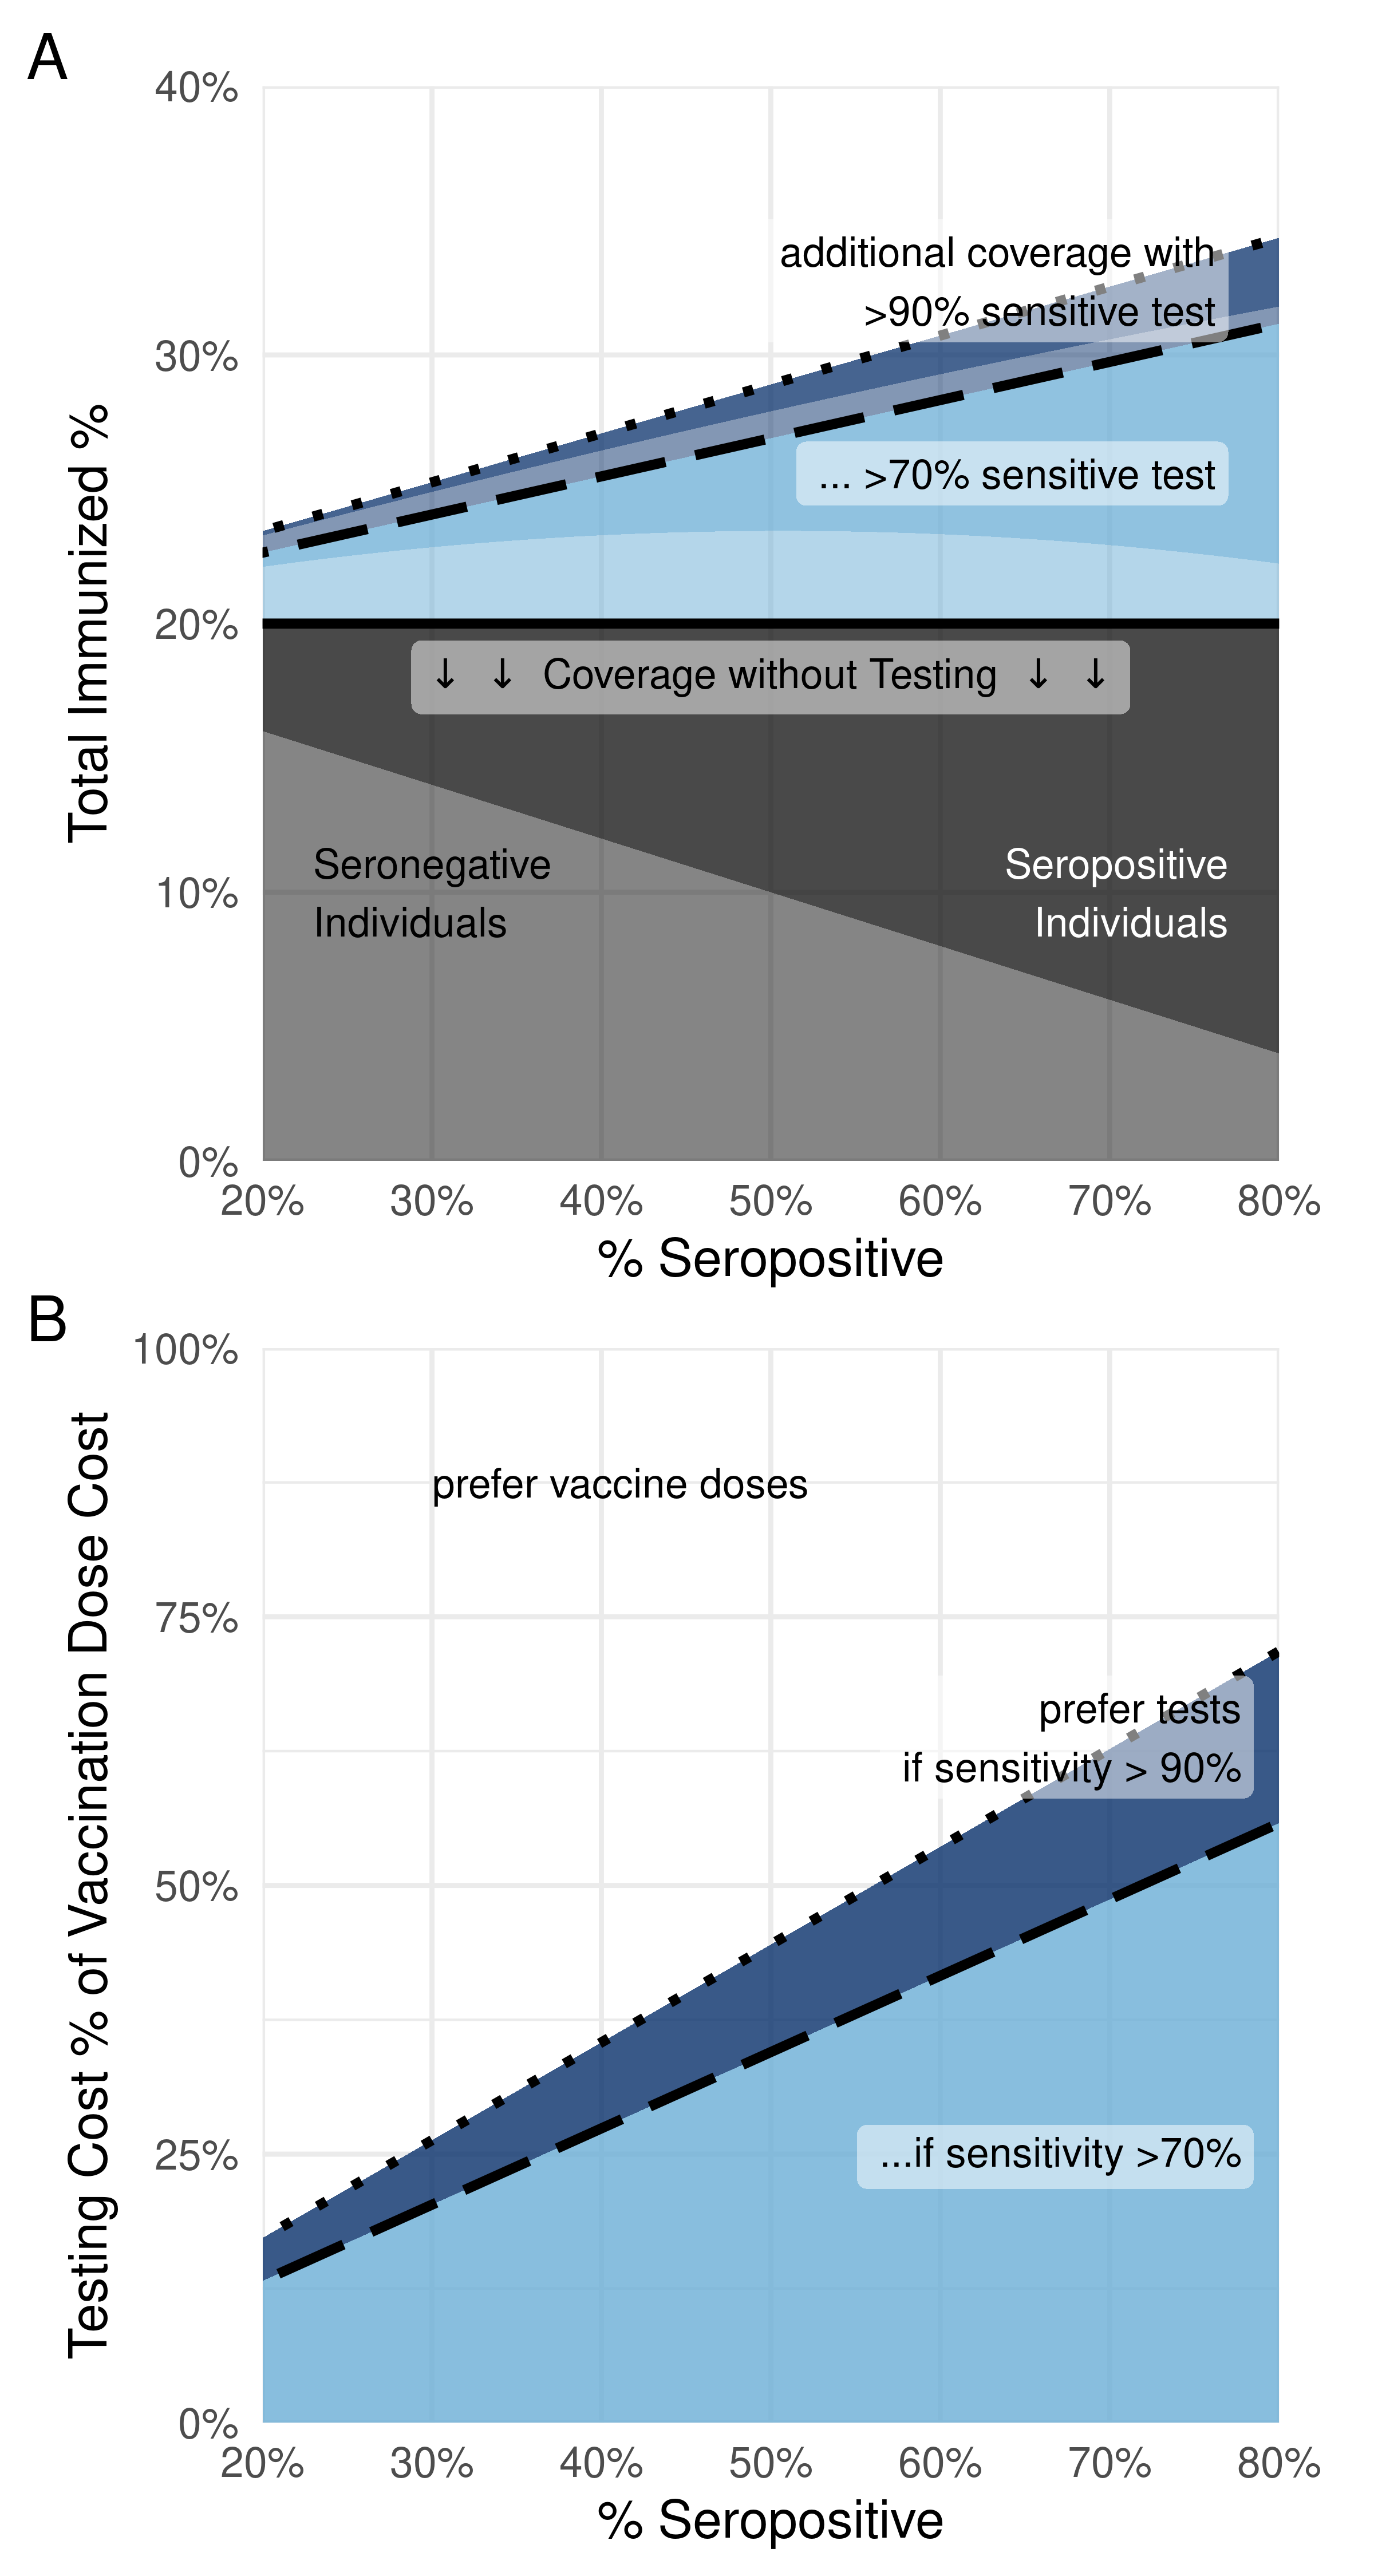
\includegraphics[width=\linewidth]{main.png}
\caption{\label{mainfig}Example Benefits of Testing. A) Assuming roughly 20\% of the population could be vaccinated without any testing \cite{noauthor_gavi_nodate}: with a highly specific test (99\%), testing can expand the percentage covered by increasing amounts depending on seroprevalence and test sensitivity (light blue: 70\% sensitive, orange: 90\% sensitivity). While many individuals still go unvaccinated, further incremental vaccine supply would result in similarly extended coverage under pre-vaccination testing approach. B) Testing can also expand the vaccinated fraction for lower costs, again depending on the vaccine-eligible population's seroprevalence and the test's performance. For a highly specific test, and relatively high seroprevalence, \eg* 40\% (dashed vertical line), a test that is less than 27\% (if >70\% sensitive) to 35\% (if >90\% sensitive) the cost of a vaccine dose is a cheaper way to expand coverage than buying more doses of vaccine. The cost advantage of testing grows with increasing seroprevalence and test performance.}
\end{figure}

\section*{Methods}

\subsection*{Coverage with Testing}

To analyze the direct benefit of this dose-sparing approach, we conservatively assume seronegative individuals are fully vaccinated (\ie* protected at the efficacy of the vaccine) only after two doses, and seropositive individuals after one dose. With a test, most seropositive individuals get one dose instead of two, freeing up doses to protect more people. Given a fixed supply, the number of additional people that could be protected depends on both test performance and the seroprevalence in the population of interest.

To evaluate this relationship, we model the population as having a homogeneous distribution of potentially test-detectable prior SARS-CoV-2 infection,  characterized by a population-level seroprevalance, $\rhop = 1 - \rhon$. We model a test that characterized by sensitivity (the true-positive rate, the complement of the false negative rate $\TPR = 1 - \FNR$), and specificity (the true-negative rate, the complement of the false positive rate $\TNR = 1 - \FPR$). For practical applications, these values will be entangled, since we know that \eg* SARS-CoV-2 antibody responses decline with time\cite{HARRIS2021}.

If we assume, pessimistically, that a single dose is not protective when given to seronegative individuals, then in our model the people protected per dose ($\PPD$) is:

$$
\PPD = 0.5*\left(\TNR\rhon + \FNR\rhop\right) + 1*\TPR\rhop + 0*\FPR\rhon
$$

which we can re-arrange in terms of complementary parameters:

\begin{equation}\label{ppd}
\begin{aligned}
2\PPD &= \left(\TNR(1-\rhop) + (1-\TPR)\rhop\right) + 2\TPR\rhop \\
&= \TNR-\TNR\rhop + \rhop - \TPR\rhop + 2\TPR\rhop \\
&= \TNR - \TNR\rhop + \rhop + \TPR\rhop \\
&= \TNR + \rhop\left(1 + \TPR-\TNR\right)
\end{aligned}
\end{equation}

Recall that without testing, two doses are required for vaccine immunity, \ie* $\PPD=0.5$. This corresponds to the situation where $\TNR=1$ (because the ``test'' is simply that everyone gets two doses) and $\TPR=0$ (because no one gets a single dose). Relative to this baseline, the relative change in $\PPD$ due to introducing testing is:

\begin{equation}\label{delppd}
\begin{aligned}
\Delta_{\PPD} &= \frac{2\PPD\left(\TNR,\TPR,\rhop\right)}{2\PPD\left(1,0,\sim\right)} - 1 \\
&= \TNR + \rhop \left(1 + \TPR-\TNR\right) - 1
\end{aligned}
\end{equation}

Assuming a single dose is non-protective in seronegative individuals helps ensure that the model represents the {\em minimal} benefit, and thus decisions continue to be beneficial even after accommodating real-world factors which are impractical to model. This limiting assumption implies that introducing testing can reduce the number of people effectively vaccinated. As practical matter, this is only a problem with extreme combinations of seroprevalence and test performance, which are not generally relevant for the settings where this scheme is worth considering. The constraining relation is $\Delta_{\PPD} > 0$ or $\TNR + \rhop \left(1 + \TPR-\TNR\right) > 1$. For example, in a population with 20\% seroprevalence, using a test with low specificity, 50\%, would be detrimental even with a perfectly sensitive test.

\subsection*{Costs}

Though testing will increase the overall cost of the vaccine program (relative to a fixed number of available vaccine doses), decision-makers should consider the cost per fully vaccinated person. One way to make that decision is to estimate which is the less expensive way to expand coverage: expanding the supply by buying more vaccine doses or more efficiently using the existing supply with testing.

We model the total cost per vaccine dose of $V$ (\ie* production, logistics, and administration) and total cost per test of $T$. On the margin, imagine purchasing one more protected person: that can be accomplished for $2V$ (\ie* two doses to get a fully vaccinated person without testing) or for some expected number of tests, $nT$, to allow re-allocation of unnecessary second doses from seropositive recipients. Restricting our consideration to situations with positive $\Delta_{\PPD}$, we can think about the relationship between $n$ and $\Delta_{\PPD}$.

If testing increases the $\PPD$ by \eg* 10\%, then using 20 tests (on average) would add another fully immunized individual. Even in situation where the test is perfect and everyone is seropositive (\ie* testing increases $\PPD$ by 100\%), two tests are still required: one to free up the second dose from an individual and one to confirm that the next recipient in line only needs one. We can generalize this relationship to $n = \frac{2}{\Delta_{\PPD}}$. Thus, using tests is preferred when

\begin{equation}\label{costlim}
\frac{2T}{\Delta_{\PPD}} \le 2V \rightarrow \frac{T}{V} \le \Delta_{\PPD}
\end{equation}

\section*{Results}

\subsection*{Expanded Coverage}

Using \eref{delppd}, we find that using a pre-vaccination antibody testing program could substantially expand vaccine coverage in populations with relatively high seroprevalence. Rearranging \eref{delppd} and considering a high specificity (99\% or $\TNR=0.99$) test, only moderate seroprevalence and sensitivity are required to observe gains: 

\begin{equation}\label{egppd}
\rhop \left(0.01 + \TPR\right) > 0.01
\end{equation}

With this high specificity and a 40\% seroprevalence \mbox{($\rhop=0.4$)} in the population of interest, only $\TPR > 0.015$ (or sensitivity of 1.5\%) is necessary to expand coverage, though of course such low performance does not expand coverage much. However, a test with sensitivity more typical of licensed medical assays (90\%) would expand coverage by 35\% (\eg* increasing a COVAX-like coverage of 20\% to 27\%). Given that the test is not needed to determine treatment, but rather more efficiently allocate doses, lower sensitivity (\eg* 70\%) might be substantially less expensive, and even that lower performance would expand coverage by 27\% (\eg* increasing a COVAX-like coverage of 20\% to 25\%). In each of the three dimensions, coverage gains increase linearly: higher seroprevalence means more opportunity to reallocate doses, higher sensitivity means taking better advantage of that opportunity, and higher specificity decreases the (assumed) loss of protection. \fref{mainfig}A shows this trend for seroprevalence (moving left to right on plot) and sensitivity (shifting from lower to higher trend lines).

\subsection*{Paying for Testing versus More Doses}

Similar to expanding coverage, using \eref{costlim}, we find that regions with relatively high seroprevalence could more effectively expand coverage with antibody testing than additional doses with a relatively high threshold for test cost. Per \eref{costlim}, the cost threshold is identical to the coverage expansion, and as such also increases linearly with seroprevalence and test performance. \fref{mainfig}B shows this trend for seroprevalence (moving left to right on plot) and sensitivity (shifting from the lower to higher shaded region).

Recalling the high seroprevalence (40\%), high specificity (99\%), and high sensitivity (90\%) scenario, the cost threshold would be 35\% of the cost of vaccination. Considering a per dose cost of roughly 15 USD (and ignoring the additional administration and logistics costs), a test that cost around 5 USD or less would be a better investment to expand coverage. Even at a lower sensitivity (70\%), the cost threshold remains plausible at 27\% of the cost, i.e. 4 USD or less per test.

\section*{Discussion \&\ Conclusions}

Where a pre-vaccination antibody testing programme is implemented, vaccine administration could be adapted to include a rapid, point-of-care antibody test before the first dose. The test result could be delivered at the end of the normal monitoring period for severe acute reactions in recipients, allowing them to be advised whether they need a follow-up dose based on their test result. For tests with imperfect specificity, some individuals with no past infection history would only receive a single dose; for our analysis, we conservatively assume these people get no protection, though studies indicate at least short-term protection \cite{krammer_antibody_2021}. Other studies have suggested that past exposure alone is sufficiently protective, and that testing could be used to administer vaccines only to seronegative individuals \cite{bubar_model-informed_2021}. While theoretically plausible, such an approach seems practically and politically untenable, could exacerbate existing inequity in COVID-19 health burdens, and does not account for potential effects like waning immunity or immune escape variants where a single dose may boost protection \cite{stamatatos_mrna_2021, lustig_neutralizing_2021}.

We have framed this analysis in terms of a population of interest. While that population could be an entire country, it could likewise be a sub-national region and/or a particular age or employment group. The pre-vaccination testing approach is most beneficial for populations with high prior burden where there is still high risk of infection, but improperly communicated could lead to the perception of these groups receiving inferior treatment and further exacerbating health inequities. While increased vaccine availability or more globally equitable distribution would reduce the need for dose-sparing methods, pragmatic solutions to expand coverage like testing may enable more efficient use in the current vaccine context. Indeed, approaches like this could be adopted in higher-income settings, where testing may require less calibration and other infrastructure advantages could offset the costs, thus freeing up vaccine supply globally.

In this analysis, we have tried to offer a conservative estimate of the potential benefits of using testing. We have focused on the directly protected individuals and the direct costs, but expanding vaccination could also increase indirect protection by reducing transmission broadly \cite{regev-yochay_decreased_2021}. Likewise, expanded vaccination could reduce the incidence of severe disease and associated costs and consumption of health service resources. We expect that a more sophisticated model incorporating these kinds of effects will predict higher testing benefits, though there are additional nuances that would dampen returns (\eg* accounting for prioritization of older populations who have high disease risk but likely lower past exposure rates). Given that our approach indicates substantial potential benefits despite being conservative, we recommend further development of rapid, point-of-care antibody testing and vaccine effectiveness studies to verify protection of seropositive individuals after single doses.

%\subsection*{Author contributions}
%In order to give appropriate credit to each author of an article, the individual contributions of each author to the manuscript should be detailed in this section. We recommend using author initials and then stating briefly how they contributed.

\subsection*{Data \&\ Software Availability}
The code for this analysis is available from \href{https://github.com/cmmid/covidTestVac}{https://github.com/cmmid/covidTestVac}.

\subsection*{Competing interests}
The authors declare no competing interests.

\subsection*{Grant information}
This research was partly funded by the Bill \&\ Melinda Gates Foundation (NTD Modelling Consortium OPP1184344: CABP), FCDO/Wellcome Trust (221303/Z/20/Z: CABP; 208812/Z/17/Z: SC), HDR UK (MR/S003975/1: RME), UK MRC (MC\_PC\_19065: RME). JRCP is supported by the South African Department of Science and Innovation and the National Research Foundation (NRF). Any opinion, finding, and conclusion or recommendation expressed in this material is that of the authors and the NRF does not accept any liability in this regard.

%\subsection*{Acknowledgements}
%This section should acknowledge anyone who contributed to the research or the article but who does not qualify as an author based on the criteria provided earlier (e.g. someone or an organisation that provided writing assistance). Please state how they contributed; authors should obtain permission to acknowledge from all those mentioned in the Acknowledgements section.
%
%Please do not list grant funding in this section.

{\small\bibliographystyle{unsrtnat}
\bibliography{refs}}

%\bigskip
%References can be listed in any standard referencing style that uses a numbering system (i.e. not Harvard referencing style), and should be consistent between references within a given article.

% Reference management systems such as Zotero provide options for exporting bibliographies as Bib\TeX{} files. Bib\TeX{} is a bibliographic tool that is used with \LaTeX{} to help organize the user's references and create a bibliography. This template contains an example of such a file, \texttt{sample.bib}, which can be replaced with your own. Use the \verb|\cite| command  to create in-text citations, like this \cite{Smith:2012qr} and this \cite{Smith:2013jd}.

% See this guide for more information on BibTeX:
% http://libguides.mit.edu/content.php?pid=55482&sid=406343

% For more author guidance please see:
% http://wellcomeopenresearch.org/for-authors/article-guidelines

% When all authors are happy with the paper, use the 
% ‘Submit to WELLCOME OPEN RESEARCH' button from the menu above
% to submit directly to the open life science journal Wellcome Open Research.

% Please note that this template results in a draft pre-submission PDF document.
% Articles will be professionally typeset when accepted for publication.

% We hope you find the Wellcome Open Research Overleaf template useful,
% please let us know if you have any feedback using the help menu above.



\end{document}